\documentclass{article}
\usepackage[spanish]{babel}
	\deactivatetilden
\spanishdecimal{.}
\addto\captionsspanish{\def\tablename{Tabla}}
\addto\captionsspanish{\def\listtablename{\'Indice de tablas}}
\usepackage[numbers,sort&compress]{natbib}
\usepackage[T1]{fontenc}
\usepackage[utf8]{inputenc}
\usepackage{graphicx}
\usepackage{url}
\usepackage{graphicx}
\graphicspath{{Figuras/}}
\usepackage[numbers,sort&compress]{natbib}
\usepackage[clearempty,pagestyles]{titlesec}
\usepackage{anysize}
\usepackage{xcolor, colortbl}
\usepackage{array, multirow, multicol}
\usepackage{enumerate} 

\def\baselinestretch{1.5}
\papersize{27.9cm}{21.5cm} 
\marginsize{2cm}{2cm}{1cm}{1cm}

\title {Algoritmo Genético}
\author{Julio Garc\'ia}
\pagestyle{empty}

\pagestyle{empty}
\begin{document}
	\renewcommand{\listtablename}{Índice de tablas}
	\renewcommand{\tablename}{Cuadro}
	\maketitle
	
	\section{Introducción}
	En el presente trabajo se busca como objetivo implementar un método de selección por ruleta para la elección de padres de un algoritmo genético. Dicha selección de ruleta toma como base una función objetivo formada por la ganancia que se tiene por los objetos contenidos en una mochila además de un inventivo por ser una solución factible. 
	
	\section{Desarrollo}
	En este trabajo se implementa un método de selección por ruleta para la elección de padres de un algoritmo genético. Dicha selección de ruleta toma como base una función objetivo formada por la ganancia que se tiene por los objetos contenidos en una mochila además de un incentivo por ser una solución factible.\\
	Además del método de selección de ruleta, se implementan también tres opciones para generar instancias. Dichas opciones están marcadas de la siguiente manera:
	\begin{enumerate}
	\item	\textbf {Opción 0}: Opción original del código para la generación de pesos y valores.
	\item 	\textbf{Opción 1}: El peso y el valor de cada objeto se generan independientemente con una distribución exponencial.
	\item   \textbf{Opción 2}:  El peso de cada objeto se generan independientemente con una distribución exponencial y su valor es (positivamente) correlacionado con el peso, con un ruido normalmente distribuido de baja magnitud.
	\item   \textbf{Opción 3}: El peso de cada objeto se generan independientemente con una distribución exponencial y su valor es inversamente correlacionado con el peso, con un ruido normalmente distribuido de baja magnitud.
	\end{enumerate}

	\section{Experimentación y resultados}
	En esta sección se describe el ambiente computacional y los resultados obtenidos con la simulación. El código de dicha simulación fue realizado en el lenguaje computacional Python en una computadora personal con procesador 1 Intel Core i7, con memoria RAM de 16GB y hasta 8 núcleos de procesamiento. Dicho código fue incorporado en el repositorio \cite{p_a}.  Se tomó como base el código de Elisa Schaeffer \cite{pa}, en el que se realizaron las variaciones requeridas.\\
	Se toman los siguientes supuestos:

		\begin{enumerate}
		\item Se realizaron experimentos para diferentes tamaños de muestra (n), dichos tamaños están calculados por $2^k$, donde $k$ está en $[2,3,4,5,6,7,8,9,10]$, no fue posible realizar experimentos con una $k$ mas grande porque la computadora no lo soportaba.
		\item  Se comparan los resultados contra el óptimo obtenido por el algoritmo exacto.
		\item   Los valores tomados para la selección en la ruleta se calculan con:
		\begin{enumerate}
		\item Suma de los valores de los objetos en la mochila + incentivo del valor máximo de los objetos siempre y cuando la solución sea factible.
		\end{enumerate}
	
		\end{enumerate}
	
    \subsection{Resultados obtenidos seleccionando padres aleatoriamente (código original)}
	
	En primer lugar, tenemos el  $\%$ de diferencia entre el optimo y la mejor solución encontrada por el algoritmo. El código original está en promedio (para las instancias generadas con las 4 opciones de generación) a $5\%$ de alejado del óptimo. Cabe mencionar que en ninguna solución con esta elección se alcanzó una solución mejor que la encontrada por el algoritmo exacto.
	
		\begin{figure}[h!]
		\centering
		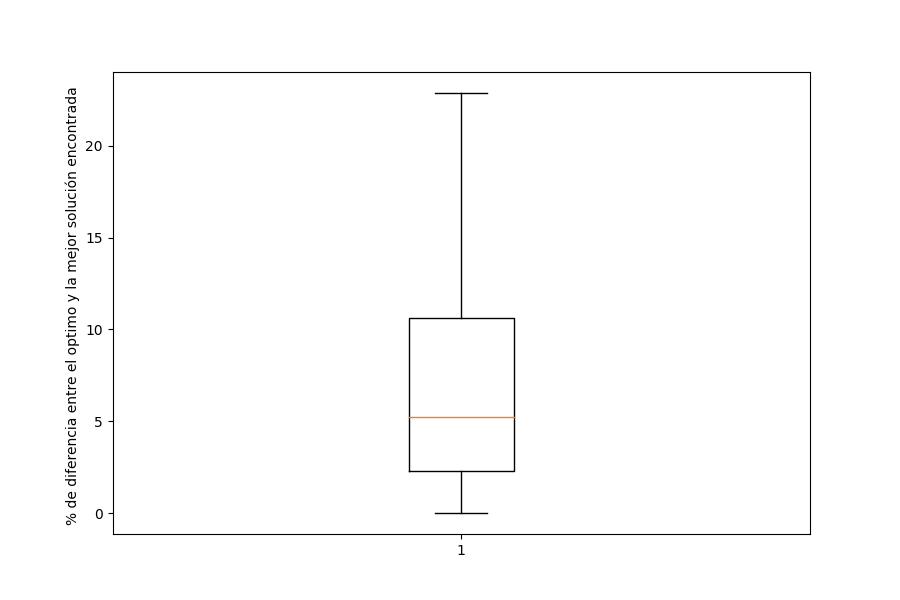
\includegraphics[width=0.7\linewidth]{Figure_1.png}
		\caption{\% De diferencia entre la mejor solución encontrada y el óptimo. Búsqueda random de padres.}
		\label{fig:imagen1}
		\end{figure}
	
	Se mide también el valor que se aporta a una función objetivo por segundo de ejecución, teniendo el siguiente diagrama.
	\newpage
		\begin{figure}[h!]
		\centering
		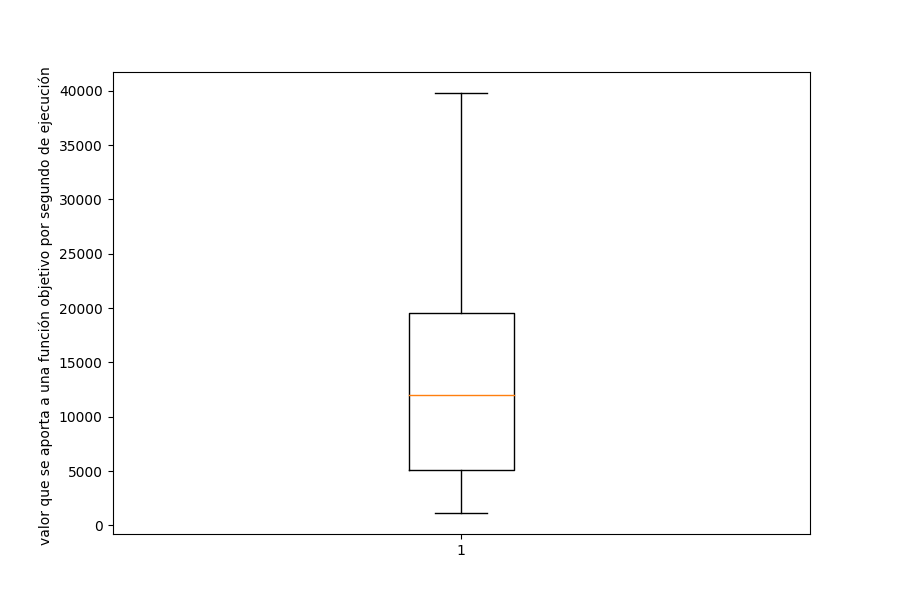
\includegraphics[width=0.7\linewidth]{Figure_2.png}
		\caption{Valor de función objetivo obtenido por segundo de ejecución. Búsqueda random de padres.}
		\label{fig:imagen2}
		\end{figure}
	
	    \subsection{ Resultados obtenidos seleccionando padres con una ruleta.}
	    
	    En primer lugar, tenemos el $\%$ de diferencia entre el optimo y la mejor solución encontrada por el algoritmo. El código original está en promedio (para las instancias generadas con las 4 opciones de generación) a $5\%$ de alejado del óptimo. Cabe mencionar en este caso, con elección de padres por método de ruleta, en una solución se alcanzó una solución mejor que la encontrada por el algoritmo exacto.
	    
	    	\begin{figure}[h!]
	    	\centering
	    	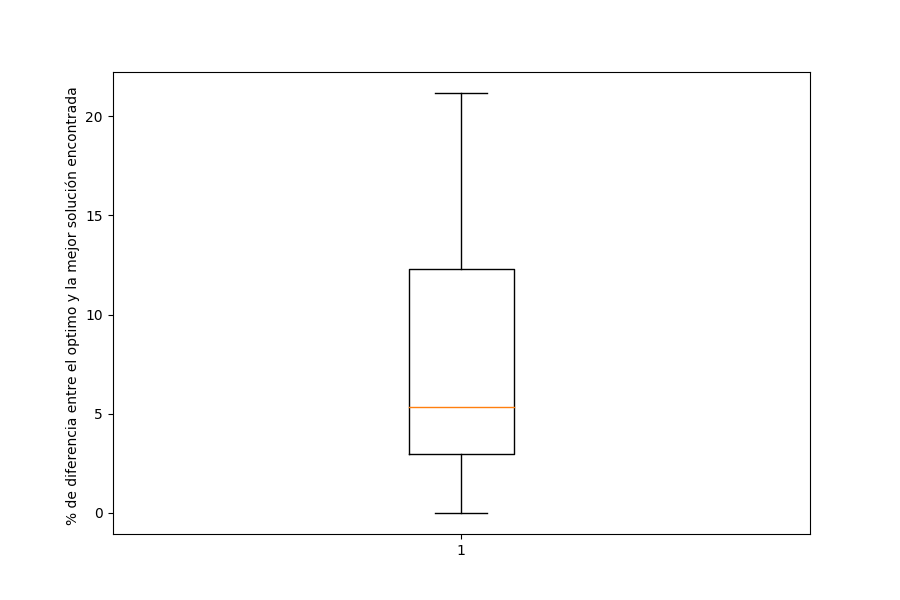
\includegraphics[width=0.7\linewidth]{Figure_3.png}
	    	\caption{\% de diferencia entre la mejor solución encontrada y el óptimo. Búsqueda de padres por ruleta.}
	    	\label{fig:imagen3}
	    	\end{figure}
    	
    	Se mide también el valor que se aporta a una función objetivo por segundo de ejecución, teniendo el siguiente diagrama.\\
    	
    	\begin{figure}[h!]
    		\centering
    		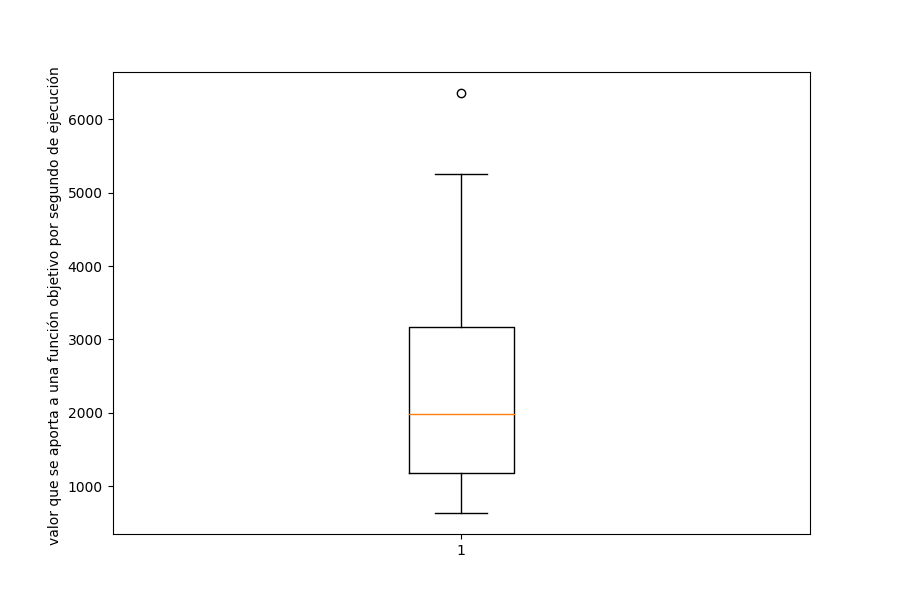
\includegraphics[width=0.7\linewidth]{Figure_4.png}
    		\caption{Valor de función objetivo obtenido por segundo de ejecución. Búsqueda random por ruleta.}
    		\label{fig:imagen4}
    	\end{figure}
    
    \section{Conclusiones}
    A continuación, se presentan las conclusiones basados en los resultados obtenidos con los diferentes métodos de selección de padres.
    \begin{enumerate}
    	\item	En cuanto a calidad de soluciones no hay una diferencia significativa entre los dos diferentes métodos se selección de padres.
    	\item	La selección de padres de manera random tiene un mejor promedio de aportación a la función objetivo por cada segundo del procesamiento, sin embargo, este indicador no da suficiente información; pudo ser por ejemplo que se generaran mochilas con mayores valores en cada producto en esta experimentación y que por eso se alcanza un mejor aporte por segundo de ejecución. 
    	\item	Valdría la pena que en el mismo experimento se seleccionara aleatoriamente uno de los dos métodos de elección de padres para posiblemente obtener mejores resultados. 
    	
    \end{enumerate}

\bibliography{Biblio}
\bibliographystyle{plainnat}

    
\end{document}